%!TEX root = ../MatMetII.tex
\chapter{Acciai per impieghi strutturali}\label{chp:AcciaiStrutturali}
Tra gli accia per impieghi strutturali, si possono trovare sicuramente gli acciai per uso comune e gli accia per costruzioni speciali: ciò per via della grande varietà di prodotti che si possono produrre in questo ambito.
Giusto per avere un'idea di massima: gli acciai per uso comune ricoprono circa l'80\% della produzione per questa categoria.
Parliamo di accia che sono designasti, in generale, tramite la lettera '\textbf{S}' secondo la normativa \ref{sc:10027-1}.

In generale sono forniti come prodotti piani e lunghi. Possono uscire in diverse forme di finitura:
\begin{itemize}
\item allo stato di lavorazione a caldo;
\item allo stato normalizzato o bonificato;
\item ecc\dots
\end{itemize}
I prodotti sono normati dalla UNI EN 10149 che è la norma prodotto di riferimento.

Come accennato esiste una normativa sulla definizione dei prodotti in acciai, distinguendo tra
\begin{itemize}
\item Prodotti piani:
	\begin{itemize}
	\item larghi piatti,
	\item lamiere,
	\item nastri,
	\item lamiere profilate (nervate, ondulate)
	\end{itemize}
\item Prodotti lunghi:
	\begin{itemize}
	\item verghelle,
	\item filo,
	\item barre,
	\item ecc\dots
	\end{itemize}
\end{itemize}

La composizione chimica si riferisce all'analisi di colata, se non diversamente specificato dalla normativa.
In generale sono descritte le $wt.\%$ massime dei vari elementi in lega, tra cui anche il carbonio, salvo specificarne diversa presenza si una piccola quantità di qualche elemento.
La norma, di solito, specifica il raggiungimento di alcune proprietà meccaniche tra cui: valori minimi di $R_s$ o $R_m$ ed eventuali caratteristiche utili al fine della costruzione come la saldabilità.
Quando è prevista zincatura per immissione a caldo di un acciaio, deve esserne garantita l'idoneità: in genere tutti gli acciai possono subire questo tipo di finitura superficiale. Però acciai adatti riescono a formare delle fasi di precipitato di zinco che garantiscono resistenza maggiorata alla corrosione ambientale. Altri, non particolarmente adatti a tale trattamento, tendono a formare delle fasi di precipitato molto irregolari e grossolane che limitano, o addirittura peggiorano, la resistenza alla corrosione.

Tipicamente, la zincabilità dipende dal contenuto in lega del Si.
Allora si possono avere diverse situazioni:
\begin{description}
\item[$Si<0.03\%$] si è in una situazione cautelativa, sicuramente si ha una buona zincatura.
\item[$0.03\%<Si<0.12\%$] È comunque zincabile, ma non ha le stesse caratteristiche di resistenza alla corrosione del primo caso. Si definiscono, dunque, delle classi di zincabilità.
\item[$Si>0.3\%$] La sequenza delle fasi di zincatura non è garantita, dunque anche la resistenza all'atmosfera non è garantita. Può migliorare la resistenza alla corrosione in maniera marginale.
\end{description}
Tra l'altro è opportuno ricordare che tale trattamento tende ad infragilire il materiale. Fenomeno esaltato dal invecchiamento.

Inoltre sono riportati all'appendice \ref{sc:AccEffCalm} la definizione degli acciai calmati ed effervescenti.

Come già accennato per questa tipologia di acciai: spesso è richiesto il soddisfacimento del requisito di saldabilità.
Viene definito un acciaio saldabile se: 

\begin{definition}{Saldabilità}{saldabilità}
Un acciaio può essere considerato saldabile se può essere sottoposto a tale processo costruttivo con le normali tecniche di cantiere senza necessità di trattamenti temici post-saldatura. 
\end{definition}

Inoltre, vale la pena ricordare che più un acciaio è temprabile, più questo sarà meno saldabile.
Questo perché un acciaio fortemente temprabile forma più facilmente strutture rigide ma fragili. Dunque un processo di saldatura, dal punto di vista del materiale, può essere considerato come una tempra con raffreddamento in aria.
In genere viene definito un parametro di carbonio equivalente detto $CEV$.
Si considera, con opportune eccezioni, saldabile un acciaio con $CEV < 0.5$.
Questo parametro non è risolutivo: qualsiasi acciaio si può saldare. Aumenta la probabilità di formare delle strutture fragili nella zona termicamente alterata $ZTA$.
In questi casi bisogna ricorrere a tecniche di saldatura più avanzate.

\section{UNI EN 10025-(3-6) Prodotti laminati a caldo}
Riprendendo la normativa UNI EN 10025 già citata al capitolo \ref{sc:10027-1}.
Si ricorda che tale normativa è dedicata a \emph{prodotti laminati a caldo per impieghi strutturali} e che è divisa in sei parti.

\begin{enumerate}
\item Condizioni tecniche generali di fornitura
\item Condizioni tecniche di fornitura di acciai non legati per impieghi strutturali
\item Condizioni tecniche di fornitura di acciai per impieghi strutturali saldabili a grano fine allo stato normalizzato/normalizzato laminato
\item Condizioni tecniche di fornitura di acciai per impieghi strutturali saldabili a grano fine ottenuti mediante laminazione termomeccanica
\item Condizioni tecniche di fornitura di acciai per impieghi strutturali con resistenza migliorata alla corrosione atmosferica
\item Condizioni tecniche di fornitura per prodotti piani di acciai per impieghi strutturali ad alto limite di snervamento allo stato bonificato
\end{enumerate}

Sono compresi nella normativa acciai di tipo \textbf{S} garantendone il valore minimo di snervamento garantito e l'indice di resilienza come indicato dalla \ref{sc:10027-1}.
In più la norma definisce ulteriori sigle per indicare l'appartenenza di tali acciai ad una ben specifica parte della normativa:
\begin{description}
\item[+AR] indica \eng{As Rolled} ovvero acciaio grezzo da laminazione;
\item[+N] acciaio proveniente da laminazione normalizzata;
\item[+M] acciaio proveniente da laminazione temomeccanica;
\item[+W] acciaio a migliorata resistenza atmosferica;
\item[+Q] acciaio ad alto valore di snervamento allo stato bonificato.
\end{description}

\begin{example}{Esempio}
Acciaio UNI EN 10025-2: \texttt{S235J0C+N} ovvero:
\begin{description}
\item[S] acciaio per impieghi strutturali
\item[235] resistenza allo snervamento minima garantita in $\unit{\MPa}$
\item[J0] resilienza garantita maggiore di $27\unit{\J}$ ad una temperatura di $0\unit{\celsius}$
\item[C] acciaio adatto per la formatura a freddo
\item[N] acciaio allo stato normalizzato
\end{description}
\end{example}

La norma definisce anche quali siano le informazioni che devono essere cedute al committente:
\begin{itemize}
\item quantitativo da fornire;
\item forma del prodotto e numero della norma per dimensioni e tolleranze;
\item Dimensioni nominali e tolleranze dimensionali di forma;
\item Designazione dell'acciaio;
\item Tipi di documenti di controllo;
\item Requisiti aggiuntivi di controllo e prova e tutte le operazioni richieste.
\end{itemize}

\begin{example}{Esempi designazione della norma}
\begin{itemize}
\item Acciaio \texttt{UNI EN 10025-3} - \texttt{S275N} o \texttt{S275NL}
\item Acciaio \texttt{UNI EN 10025-4} - \texttt{S420M} o \texttt{S420ML}
\item Acciaio \texttt{UNI EN 10025-5} - \texttt{S355J0W+N} o \texttt{S355J0WP+N}
\item Acciaio \texttt{UNI EN 10025-6} - \texttt{S460Q} o \texttt{S460QL} o \texttt{S460QL1}
\end{itemize}
\end{example}
L'indice \texttt{L} indica valore di resilienza minima garantita più alta rispetto al solo parametro \texttt{N} a diverse temperature.
Stesso discorso per i parametri \texttt{M} e \texttt{ML} Solo che la condizione finale di fornitura è diversa.
Mentre per gli acciai che presentano il temine \texttt{W} o \texttt{WP} hanno dei tenori di Cr e Cu ben specificati dalla normativa. Quindi indicano una diversa composizione di lega.

\section{Acciai resistenti alla corrosione atmosferica}
Sono commercialmente definiti come acciai \textbf{Cor-Ten} che sta ad indicare:
\begin{description}
\item[\eng{Cor}] "\eng{Corrosion resistance}"
\item[\eng{Ten}] "\eng{Tensile strength}"
\end{description}

Per aumentare la resistenza atmosferica contengono come elementi in lega:
Cu, Cr, Ni e in caso tenori variabili di P.
La composizione tipica potrebbe essere:
\begin{example}{Composizione tipica CORTEN}
\begin{tabularx}{\textwidth}{XXXXXXX}
\toprule
C & Mn & Si & Cr & Ni & Cu & V\\
0.15 & 1.10 & 0.80 & 0.50 & 0.70 & 0.30 & 0.05\\
\bottomrule
\end{tabularx}
\end{example}
In genere questi acciai vengono forniti allo stato di laminazione di
normalizzazione o semplicemente laminato. Oppure sotto forma di barre, 
profilati e lamiere.
Altre normative descrivono questi acciai come adatti per applicazioni architettoniche ed eventualmente adatti per applicazioni più sollecitate.

Sono acciai che generalmente sono saldabili, eventualmente il materiale
di apporto che vengono usati anche per acciai Cr-Mn. Nel caso sia
necessaria una certa finitura estetica (caso di applicazioni
architettoniche) si usano elettrodi contenenti del Ni ($\approx 2 \div 
3\%$) per ottenere la stessa finitura superficiale.

\section{Acciai ad alta resistenza (HSS e AHSS)}
Sono acciai che hanno un preciso scopo: garantire alte prestazioni 
meccaniche senza eccedere con elementi leganti per mantenere un costo 
del materiale alto.
In particolare, le caratteristiche da ricercare in questo acciaio sono:
\begin{itemize}
\item Carico di rottura
\item Carico di snervamento
\item tenacità
\item talvolta una migliorata resistenza alla corrosione 
atmosferica e alle atmosfere industriali (potenzialmente 
aggressive)
\end{itemize}
Lo sviluppo degli acciai \textit{micro-legati} ha consentito
alla realizzazione di dimensionamenti a minore quantità di materiale
senza perdere di tenacità e duttilità ed altre caratteristiche
meccaniche.
Inoltre la micro-legatura ha tolto la necessità di
eseguire dei trattamenti termici successivi. Che ovviamente
si traduce per entrambi gli scopi in minori costi di produzione.

\subsection{Meccanismi di rinforzo}
Per raggiungere gli obbiettivi indicati in precedenza, gli acciai 
ad alta resistenza presentano i così detti \emph{Meccanismi di rinforzo}.
Si vedranno ora i principali.

\paragraph{Rafforzamento per soluzione solida}
Si tenda ad aumentare il tenore di carbonio, così il materiale diventa
più duro. In più, si sostituiscono gli elementi sostituzionali: tali 
deformano il reticolo cristallino interagendo con le dislocazioni, di 
fatto bloccandole.

\paragraph{Incrudimento}
La semplice lavorazione a freddo porta il materiale ad incrudire, 
per cui risulta più duro. Ciò è dovuto all'aumento delle dislocazioni.

\paragraph{Rinforzo per precipitazione}
Vengo costituite, tramite opportuni processi produttivi, delle fasi
solide sovrassature che pongono un ostacolo al movimento delle
dislocazioni.

I metodi presentati in precedenza, sebbene migliorino la resistenza
in generale, costituiscono un problema in termini di duttilità:
Andando a bloccare le dislocazioni si ha effettivamente un materiale
più duro, al contempo si perde di duttilità.
Alla figura \ref{fig:RinfTenacita} sono riportati qualitativamente.

\begin{figure}
\centering
\subfloat[][\emph{Effetti negativi}\label{fig:EffettiNegativiRinforzo}]
{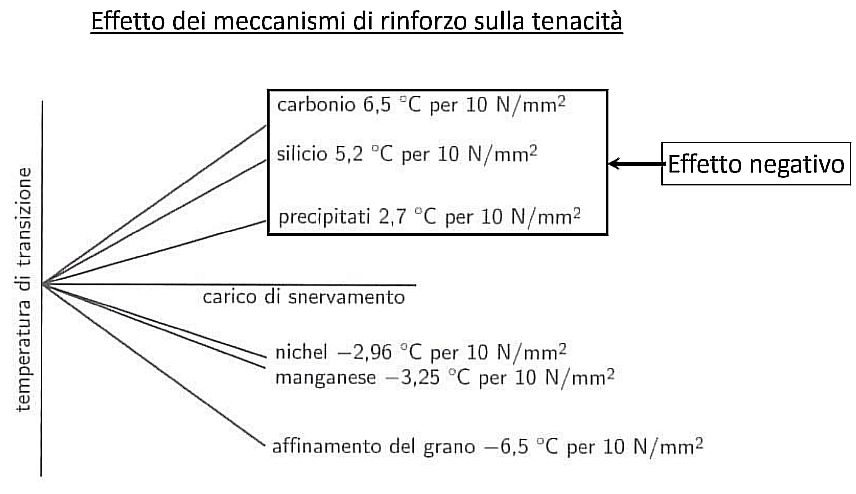
\includegraphics[width = 0.4\textwidth]{EffettoRinforzoTenacita}} \quad
\subfloat[][\emph{Effetti positivi}\label{fig:EffettiNegativiRinforzo}]
{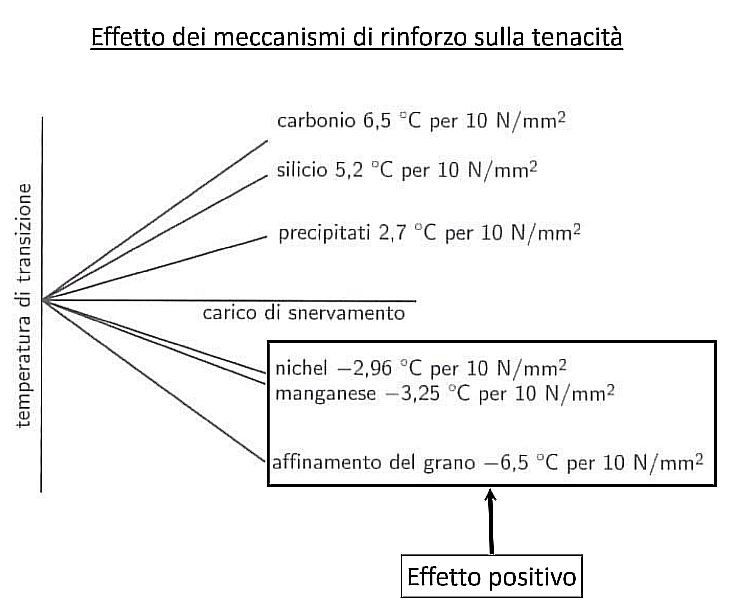
\includegraphics[width = 0.4\textwidth]{EffettoRinforzoTenacita2}}
\caption{meccanismi di rinforzo in rapporto alla tenacità}
\label{fig:RinfTenacita}
\end{figure}

\paragraph{Rafforzamento per affinamento del grano}
Nel caso di strutture cristalline CCC, come per acciai 
ferritico-perlitici per costruzione saldate, è l'unico meccanismo 
che incrementa entrambe le qualità: resistenza e tenacità.
Allora valgono:
\begin{align}
R_s &= \sigma_0 + K d^{-1/2} \label{eqn:tensServ}\\
I.T.T. &= A - B \ln d^{-1/2} \label{eqn:ITT}
\end{align}
Dalla \eqref{eqn:tensServ} e \eqref{eqn:ITT} è evidente come le 
dimensioni dimensioni del grano siano fondamentali per controllare
contemporaneamente la tensione di snervamento e la \eng{Input 
Transition Temperature}. Nello specifico:
\begin{equation}
\searrow d \Rightarrow \nearrow R_s \text{ e } \searrow I.T.T.
\label{eqn:RelMigli}
\end{equation}

\begin{figure}
\centering
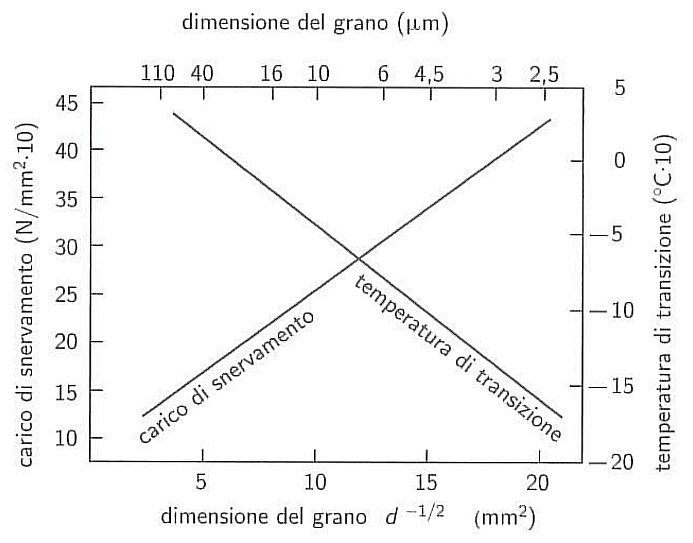
\includegraphics[width = \textwidth]{MiglDimGrano}
\caption{Miglioramento tramite dimensione del grano}
\label{fig:MiglDimGrano}
\end{figure}

\begin{center}
\emph{Come si può controllare le dimensioni del grano ferritico?}
\end{center}
In genere non è sempre possibile agire sulla velocità di raffreddamento, 
perché nella laminazione a caldo, il raffreddamento, vine eseguito in 
aria. Perciò dipende dallo spessore del laminato.
Allora si può controllare la dimensione del grano austenitico durante 
la permanenza ad alta temperatura.
Perché il grano ferritico nuclea a bordo del grano austenitico, quindi 
se si limitano le dimensioni dell'austenite se ne limita la nucleazione
in ferrite, almeno diemensionalmente parlando.
Inoltre si può ricorrere all'aggiunta in lega di microleganti
che formano dei carburi i carbonitruri che "fissano" il grano
austenitico impedendone la crescita.

Da queste considerazioni si sono sviluppati gli \texttt{HSLA} ovvero
acciai ad alta resistenza ma basso legati.

\subsection{HSLA}
Gli \ac{HSLA} sono acciai con un prezzo più vicino a quello degli acciai 
al carbonio per via del fatto che non contengono tenori di elementi in 
lega eccessivamente alti. Inoltre la loro produzione non è eccessivamente 
costosa per via dei sistemi di rinforzo che sono stati accennati in 
precedenza.

Generalmente ne esistono diverse categorie perché sono venduti in base
alle loro caratteristiche meccaniche piuttosto che sulla composizione
chimica:
\begin{itemize}
\item Acciai a migliorata resistenza alla corrosione atmosferica
\item Acciai microlegati ferritico-perlitici
\item Acciai con ferrite aciculare
\item Acciai con morfologia controllata delle inclusioni
\end{itemize}

I primi ad essere stati considerati come \ac{HSLA} sono stati i 

\subsubsection{Ferritico-Perlitici ad alta resistenza}
Il loro sviluppo è stato possibile grazie all'introduzione della laminazione in controllo.

\begin{definition}{Laminazione in controllo}{*}
Deformazione a caldo con controllo accurato della temperature,
in modo da bilanciare l'effetto dell'affinamento del grano per
deformazione con quello della ricristallizzazione dovuta alle 
alte temperature.
\end{definition}

L'evoluzione di questi saranno gli acciai ferritico-perlitici
ad alta resistenza e tenacità.

Sono acciai che contengono V e Nb come elementi microalliganti.
Per questi acciai le temperature di fine laminazione dono in genere 
superiori ai $900\unit{\celsius}$ e il raffreddamento avviene in
aria calma.
Si ottiene, dunque, un acciaio con grano ferritico non in controllo ma
rinforzato dai carburi dei microlegati.
\begin{description}
\item[Acciai al niobio] interessa la precipitazione dei carburi NbC,
\item[Acciai al vanadio-azoto] interessa la precipitazione dei nitruri
VN.
\end{description}

\begin{figure}
\centering
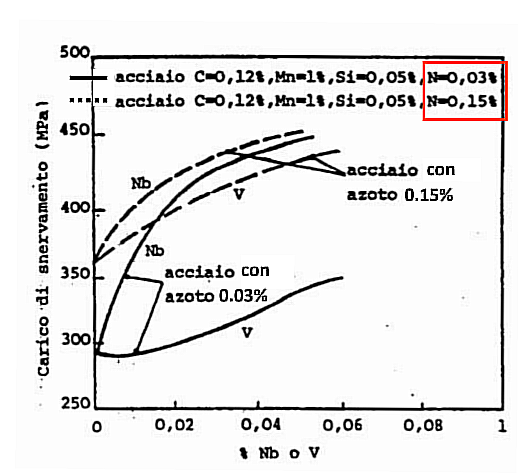
\includegraphics[width = \textwidth]{FerPerHS}
\caption{Variazioni dello snervamento con l'aggiunta di microleganti}
\label{fig:FerPerHS}
\end{figure}

Dalla figura \ref{fig:FerPerHS} si evidenzia come per acciai microlegati
al Nb l'effetto del azoto sia indifferente. Già più marcato per gli 
acciai al V. Questo perché si formano i nitruri di vanadio.
Da notare come a parità degli altri leganti, gli acciai che presentano
microleganti ottengano una tensione di snervamento decisamente migliore.
Si vuole ricordare che non sono state eseguite operazioni di affinamento 
del grano, si considera infatti una dimensione del grano pari a $d 
\approx 14 \div 16\unit{\um}$.

Ulteriore miglioramento delle caratteristiche di snervamento si 
raggiunge nel caso di aggiunta di $1\%Cu + 1\%Ni$.
Il rame è poco solubile col ferro al diminuire della temperatura.
Se il materiale viene raffreddato molto rapidamente, il rame tende a 
rimanere in soluzione solida sovrassatura.
Operando un rinvenimento a $\approx 550\unit{\celsius}$ si ha la 
precipitazione della fase $\epsilon$ con ulteriore rafforzamento per 
precipitazione.
Rafforzamento inizialmente possibile solo per lamiere.

\subsubsection{Ferritico-Perlitici ad alta resistenza e alta tenacità}
Sono comunque acciai microlegati con cui si procede con 
\textbf{Affinamento del grano}, controllato tramite controllo della
dimensione del grano austenitico di partenza.
Grazie a questo processo si ha un miglioramento della tenacità.
Dopodiché si hanno duo possibili vie per migliorare anche la resistenza:
\begin{enumerate}
\item \textbf{Normalizzazione}, in genere più adatta per lamiere con 
spessore $>25\unit{\mm}$;
\item \textbf{Laminazione controllata} per lamiere di spessore 
$<25\unit{\mm}$.
\end{enumerate}

\paragraph*{Normalizzazione} per lamiere di spessore $>25\unit{\mm}$
In questo caso si segue un procedimento del tipo proposto alla figura \ref{fig:NormFerPer}.
I dettagli delle operazioni post laminazione a caldo saranno:

\setlength{\columnsep}{35pt}
\begin{multicols}{2}
\begin{definition}{}{*}
T finale di laminazione $> 900 \div 1000\unit{\celsius}$
\end{definition}
L'austenite non diventa sovrassatura degli elementi microlegati.
Dunque non si ha precipitazione di carburi per difficoltà nella
nucleazione. Abbassando la temperatura l'austenite cristallizza quando
il grano non è in controllo. Si andrà a generare un grano ferritico non 
particolarmente fine però rinforzato dai precipitati.
In generale si avrà \textbf{una resistenza non particolarmente alta e
tenacità scadente}.
\columnbreak
\begin{definition}{}{*}
T finale di laminazione $> 880 \div 900\unit{\celsius}$
\end{definition}
I carburi precipitano mentre l'austenite tende a riscristallizzare, dunque
ne controllano la crescita.
I precipitati devono essere molto fini e dispersi, altrimenti 
infragiliscono la struttura.
Si genererà un grano ferritico con $d \approx 5 \div 6\unit{\mm}$ con 
contributo di $R_s = 390\div450\unit{\MPa}$.
Aggiungendo il contributo dato dai precipitati si arriva a $R_s = 
550\unit{\MPa}$. Ottenendo \textbf{resistenza e tenacità più alte}
\end{multicols}

\begin{figure}
\centering
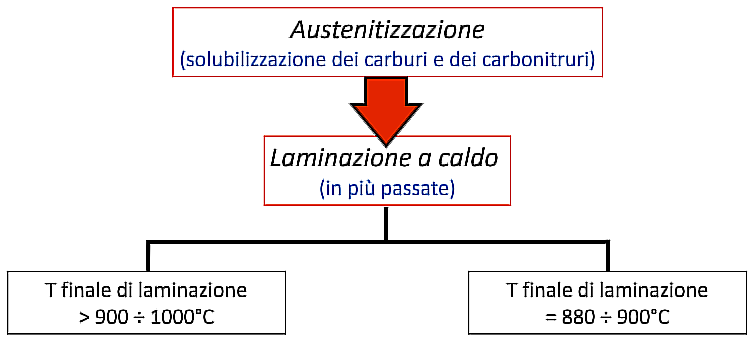
\includegraphics[width = \textwidth]{NormFerPer}
\caption{Possibilità sul trattamento di normalizzaizone}
\label{fig:NormFerPer}
\end{figure}